\documentclass[11pt]{article}
\usepackage[UTF8]{ctex}
\usepackage[a4paper,left=25mm,right=25mm,top=25mm]{geometry}
\usepackage{xeCJKfntef}
\usepackage{amsmath,amsfonts,amssymb}
\usepackage{tikz}
\usepackage{pifont}
\usepackage{subfigure}
\usepackage{caption}
\usetikzlibrary{arrows.meta}
\renewcommand{\figurename}{}
\renewcommand{\thesubfigure}{}
\makeatletter \renewcommand{\@thesubfigure}{\thesubfigure \space}
\renewcommand{\p@subfigure}{} \makeatother
\begin{document}
\begin{figure}[h]
    \raggedleft
    \subfigure[(第22题)]{
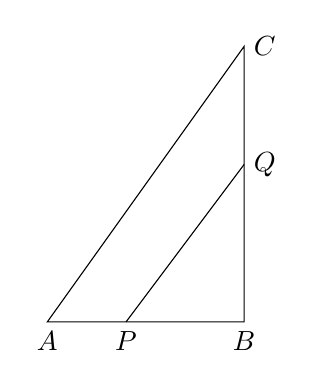
\begin{tikzpicture}[scale=0.5]
    \node[below] at (-5,0) {$A$};
    \node[below] at (0,0) {$B$};
    \node[right] at (0,7) {$C$};
    \node[below] at (-3,0) {$P$};
    \node[right] at (0,4) {$Q$};
    \draw (-5,0)--(0,0)--(0,7)--cycle;
    \draw (-3,0)--(0,4);
\end{tikzpicture}}
\end{figure}
\end{document}